%   TNT user-guide
%
%  This latex document is the TNT 1.x users guide.
%  It can be compiled into ps, pdf, and html formats.
%  Online help could use the html format.
%
%  Copyright (C) 2004 by Mayo Foundation.  All rights reserved.
%
%  Bob Techentin
%  June 23, 2004
%
%  $Id: user-guide.tex,v 1.5 2004/07/26 13:39:09 techenti Exp $
%


\documentclass{article}

%
%  Use amsmath, because mathematics will be beautiful.
\usepackage{amsmath}
%
%  Set up graphicx package to include screen pictures,
%  with maximum size of the line width.  Some smaller
%  screen pictures use fractions of \linewidth, which
%  doesn't affect latex2html.  
%  Hmmm.  Seem to get good results with scale=0.5
%  on the original screen captures, but that doesn't
%  work with this global technique.  
\usepackage{graphicx}
%\setkeys{Gin}{width=0.8\linewidth}
%
%
%  Use html, for image inclusion in html format
%  and generating bookmark table of contents in pdf.
\usepackage[plainpages=false]{hyperref}
\usepackage{html}
%
%
%  Set title for Table of Contents (default is ``Contents'')
%  Also correct sizes from ``\HUGE'' in report style
\renewcommand{\contentsname}{\large{Table of Contents}}
\renewcommand{\listfigurename}{\large{List of Figures}}
%\renewcommand{\bibname}{\large{Bibliography}}
%

\usepackage{fancyhdr}
\pagestyle{fancy}


\title {TNT 1.2 Users Guide}

\author {
Bob Techentin \\
Mayo Special Purpose Processor Development Group}

\begin{document}

\maketitle


%-----------------------------------------------------------
%  Automatic Tables of Contents and Figures
%-----------------------------------------------------------
\clearpage
\pagenumbering{roman}
\tableofcontents
\clearpage
\listoffigures
\clearpage
\pagenumbering{arabic}

%-----------------------------------------------------------
%  Abstract
%-----------------------------------------------------------
\addcontentsline{toc}{section}{\numberline{}Abstract}
\begin{abstract}

This users' guide describes the TNT transmission line modeling
software package.  The software was developed by the Special Purpose
Processor Development Group, a research group at Mayo Clinic in
Rochester Minnesota.  This guide describes installation and operation
of the TNT graphical user interface, and the MMTL and Wavelet
simulators.


\end{abstract}

\clearpage
\setcounter{page}{2}


%-----------------------------------------------------------
%  Numbered sections and subsections are the body of the document
%  Every section should include both a title and a label, so
%  that it can be referred elsewhere in the paper.
%-----------------------------------------------------------

\section {Introduction}

The TNT software package was developed by the Special Purpose
Processor Development Group (SPPDG) at Mayo Clinic in Rochester
Minnesota.  TNT was created in an effort to simplify and unify
transmission line modeling for high performance electronics system
designs.  The SPPDG has developed and used several different
transmission line ``field solvers.''  Each tool had unique
capabilities and limitations, and each tool had a different and often
complex user interface.

TNT makes it very simple to create and modify two dimensional cross
section descriptions of transmission line interconnect structures.
The transmission line is represented as a cross section, with ground
planes, dielectric layers, and conductors.  Cross sections can be
saved in a format called the Cross Section Description Language, which
can easily be edited, customized, or even programmed.

TNT also makes it easy to run the electromagnetic field solvers which
generate per-unit-length transmission characteristics.  TNT is
integrated with the Multilayer Multiconductor Transmission Line (MMTL)
quasi-static simulator and two experimental wavelet-based full-wave
transmission line analyzers.  All simulators can be run simply from
the TNT menus.  MMTL can be run iteratively by sweeping cross section
parameters or by iterating until a desired characteristic impedance is
achieved.


%-----------------------------------------------------------
%  License
%-----------------------------------------------------------

\section {License and Warranty}

You are licensed to use, copy, modify, and share the TNT software
package according to the terms of the GNU General Public License.  The
license terms are in the file COPYING included with TNT.

Under the General Public License, you may install and use TNT on any
number of computers.  You may examine the source code of the program
to determine how it works.  You may modify the program, hopefully
making it better, and you may share the program with others.  If you
make improvements to TNT, we would appreciate it if you let us know.

Like most software, TNT comes with absolutely no warranty.
Fortunatley, if there are problems, you are allowed to examine the
source code, recompile the program, and correct the problem.

There are some software components included with TNT that are licensed
separately.  Printing on Microsoft Windows requires, for example, a
print utility by Peter Lerup, which is licensed under terms described
in the documentation in printfile215-32.zip.  Tcl, Tk, and extensions
are licensed under terms similar to those of the Berkely license,
which imposes fewer obligations on the user than the GPL.  Please
refer to each package's license information.


%-----------------------------------------------------------
%  Installation
%-----------------------------------------------------------

\section {Installation}

TNT is free software.  You can compile it from source code, or you can
install a pre-compiled binary distribution.  While most
Windows users expect a binary distribution, many Unix or
Linux users can build and install from sources.  This section will
describe both approaches.

TNT was originally developed to run on SPPDG workstations running
HP-UX, and depends on several packages that are installed and
maintained a the SPPDG.  TNT has been ported to Linux and
Windows, and an installation kit produced which should
make it relatively straight forward to install the software on similar
workstations or PCs.


\subsection {Tcl/Tk and Other Dependencies}

TNT requires a functional installation of Tcl and Tk with several
extensions, including BWidget, Incr Tcl, and Iwidgets.  You
will need to install all of these packages in order for TNT to
function correctly.  TNT expects to be able to find the {\tt wish}
windowing shell in your command path.

You {\em could} compile and install these packages from the freely
available source code hosted at Sourceforge.  Specifically, you can
acquire them from http://tcl.sf.net/, http://tcllib.sf.net/, and
http://incrtcl.sf.net/.  You will need an ANSI C compiler, such as the
GNU Compiler Collection from http://gcc.gnu.org.  You should be able
to use the Microsoft Visual C++ compiler or MinGW for Windows systems.
You may find this an enjoyable challenge, or, if you are not a
programmer, you might find the process difficult and frustrating.

Alternatively (and highly recommended), you can install a freely
available, pre-compiled Tcl and Tk package from ActiveState, which
includes all these extensions.  The ActiveTcl distribution is, in
fact, installed on SPPDG workstations and PCs.  Unfortunately, while
the ActiveState packages are free to use, we are not permitted to
distribute the packages with TNT.  You can obtain ActiveTcl for
Windows, Linux, Solaris, or
HP-UX from http://www.activestate.com/.



\subsection {Microsoft Windows Installation}

\subsubsection {Windows and Tcl/Tk}

The Windows distribution includes a Tcl/Tk runtime along with
all the extensions necessary to run the application.  So you don't
really need to download and install ActiveTcl or other Tcl/Tk
distributions to make TNT work on your PC.  But Tcl is so much 
fun to use, that you really ought to consider getting a copy.


\subsubsection {Windows and TNT} \label{sec:win-install}

TNT has a basic Windows installation program.  Just click on the
installer file, accept the GPL license, specify an installation
location, and let it do the work.  Installing TNT does not require
administrative priviledges on Windows 2000 or Windows XP, but if an
administrator performs the installation, then the package will be
available for all users.

The installation program will create a shortcut to run TNT.  You may
want to copy that shortcut, and modify the ``Start In'' directory to a
location where you normally work with transmission line simulations.

\subsection {UNIX Installation}

\subsubsection {UNIX and Tcl/Tk}

Download and install ActiveTcl from http://www.activestate.com/.  This
gets you Tcl, Tk, BWidget, Incr Tcl, Iwidgets, and a lot of other cool
stuff.


\subsubsection {UNIX and TNT}

If you have a binary distribution, just copy the TNT directory tree
from the installation kit to a location from which applications are
normally run.  This could be {\tt /usr/local/} or a personal
subdirectory or some other location.  Make sure that the directories
for {\tt wish} and {\tt .../tnt/bin} are in your path.

To build TNT from sources, unpack the source code distribution
archive, and follow the instructions in the file named INSTALL.


%-----------------------------------------------------------
%  Starting TNT
%-----------------------------------------------------------

\section {Starting TNT}


On Windows, the TNT program is run by clicking on the menu item or
shortcut that you created in \ref{sec:win-install}.  Alternatively,
you can use Windows Explorer to navigate directly to the TNT
installation directory, and click on {\tt tnt.tcl}.

On Unix, the program is invoked at the command line by executing
either "tnt" or "tnt.tcl" from the installation directory.  If the
binary directory {\tt .../tnt/bin} is included in your path, simply
type the command.  Otherwise, you may specify a full path name to {\tt
tnt.tcl}, or you can change your current working directory (cd) to the
{\tt .../tnt/bin} directory, and run the application from there.

When started, TNT will not have any simulation parameters defined.
You may use the {\bf Open}, {\bf Save}, and {\bf Save As...} options
from the {\bf File} menu to load and save TNT cross section files.

\subsection {TNT Main Window}

The TNT main window contains an application menu bar, buttons for
creating new cross section structures, a layer stackup, and a drawing
of the cross section.

\begin{figure}[hbt]
\begin{center}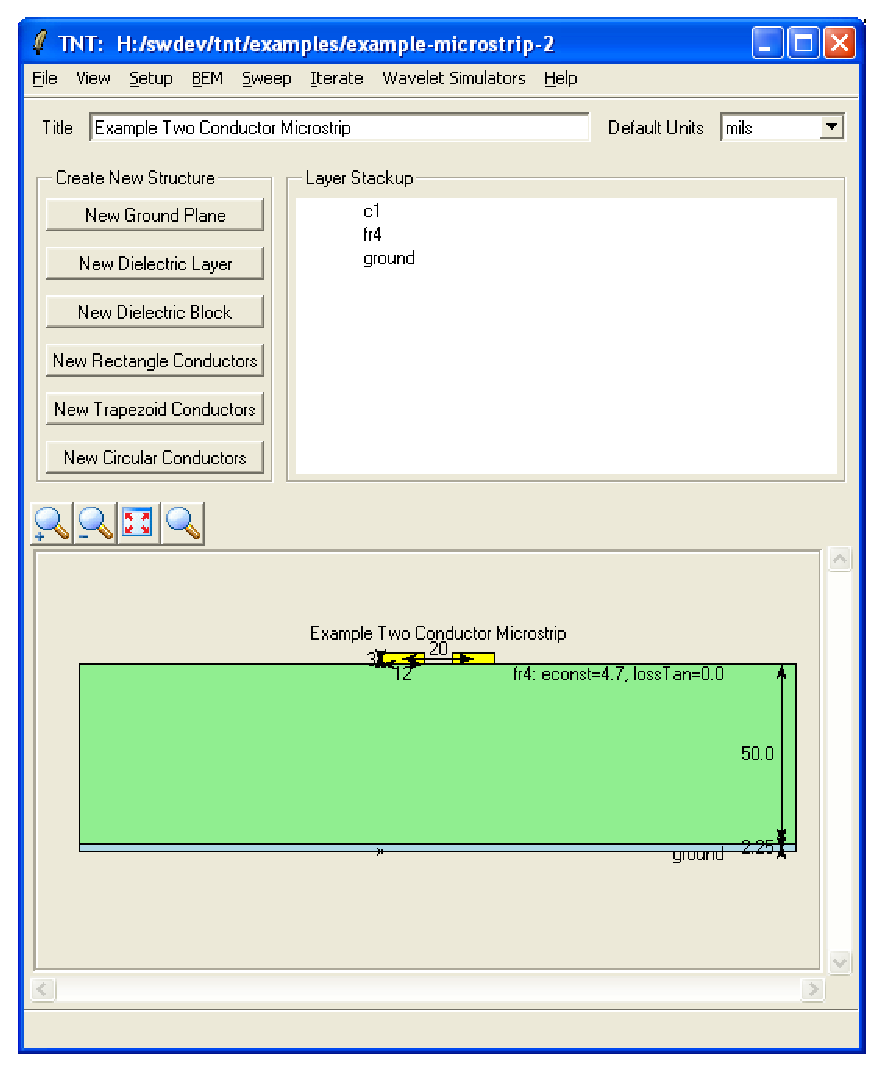
\includegraphics[scale=0.5]{mainwindow}\end{center}
\caption { TNT Main Window }
\label{fig:mainwindow}
\end{figure}


The menu bar has several pull-down menus.  The {\bf File} menu has
options for opening, saving, and printing cross section description
files.  The {\bf View} menu toggles display options.  Materials lists
can be re-loaded using options on the {\bf Setup} menu.  MMTL
simulations can be run from the {\bf BEM}, {\bf Sweep}, and {\bf
Iterate} menus.  The full-wave experimental wavelet based simulators
can be run from the {\bf Wavelet Simulators} menu.



%-----------------------------------------------------------
%  Cross Sections
%-----------------------------------------------------------

\section {Cross Sections}


%-----------------------------------------------------------
%  Example Cross Sections
%-----------------------------------------------------------

\subsection {Example Cross Sections} \label{sec:examples}

You can create a cross section from scratch, as described in
section~\ref{sec:create}, or you can start with one of the example
cross sections that is distributed with TNT, and modify it according
to your needs.

The example cross sections are in the TNT installation directory,
under {\tt .../TNT/examples}.  Choose {\bf File $\Rightarrow$ Open}
from the menus, navigate to the example directory, and choose one of
the cross section files.  You may then modify it and save it elsewhere
with {\bf File $\Rightarrow$ Save As}.




%-----------------------------------------------------------
%  Creating a Cross Section
%-----------------------------------------------------------

\subsection {Creating a Cross Section} \label{sec:create}

To create a new cross section, you can choose {\bf File $\Rightarrow$
New} from the menu.  This will clear any existing structures from the
layer stackup and the drawing window.

Enter a model title in the {\bf Title} field.  The model title should be
descriptive, and will be saved with the cross section model.  Set the
units to match the physical dimensions of your transmission line
structure.

Start adding structures to the layer stackup by creating a ground
plane, then adding layers of dielectrics and conductors.  Clicking on
the {\bf New Ground Plane} button will open a new window allowing you
to define the structure name and the thickness.  Clicking {\bf Add} on
the dialog will add the ground plane to the layer stackup and the
drawing.

Continue by adding dielectric layers.  Click on the {\bf New
Dielectric Layer} button to open the dielectric properties entry form.
Each layer has a name, thickness and material characteristics.  Make
sure that the default units selected at the top of the screen match
your intentions for the layer dimensions.  (You don't really want a 42
meter thick dielectric, do you?)

Layers will appear in the cross section drawing as you add them, and
layer names will appear in the layer stackup.  If you do not add a top
ground plane (i.e., microstrip), then air is assumed to be above the
top defined layer.

Add conductors to the cross section by selecting one of {\bf New
Rectangle}, {\bf Trapezoid}, or {\bf Circular Conductors} buttons,
which will open a new properties dialog for the conductors.  Each
conductor structure has dimensions and material properties.  When you
{\bf Add} these conductors, they will rest atop the last defined
dielectric layer.  You can add a single conductor, or a group of
identical conductors with a specified pitch.  You can specify X and Y
offsets to the conductors.

You can also define {\bf New Dielectric Block}s which are arbitrary 
rectangles of dielectric material.  These blocks can be used to define
non-planar (conformal) dielectric structures.


%-----------------------------------------------------------
%  Modifying a Cross Section
%-----------------------------------------------------------

\subsection {Modifying a Cross Section} \label{sec:modify}

Select cross section elements by clicking on them either in the {\bf
Layer Stackup} window or on the cross section drawing.
Double-clicking on a cross section element opens its properties
dialog.  You can choose to {\bf Modify} the properties or {\bf Delete}
the structure.

You can rearrange the order of the layer stackup by clicking and
dragging structures in the {\bf Layer Stackup} window.

The cross section drawing is supposed to give you a graphical
depiction of your transmission line cross section.  Unfortunately, the
scale of many conductor definitions makes it difficult to see the
drawing easily.  You may need to use the zoom buttons to get a better
view of the structures.


%-----------------------------------------------------------
%  Printing
%-----------------------------------------------------------

\subsection {Printing}

You can print the cross section picture on a postscript printer by
choosing {\bf File $\Rightarrow$ Print} from the menu.  The print
dialog offers several options, including paper size, orientation, and
output specification.

On Unix systems, the default printer command is {\bf lpr}, which
should work for most installations.  Choose a different print command,
or add options, if you choose.  On Windows systems, the default
printer command is {\bf PrFile32.exe}, which is a small utility
program that directs the postscript to a Windows print queue.  If you
do not have a postscript printer, you will likely get many pages of
printed postscript commands.



%-----------------------------------------------------------
%
%  BEM MMTL
%
%-----------------------------------------------------------

\section {BEM MMTL}

The Boundary Element Method (BEM) Multilayer Multiconductor
Transmission Line (MMTL) simulator is the most recent of several
generations of electromagnetic modeling packages developed at the
SPPDG.  This program uses the Method of Moments (MOM) technique to
quickly compute capacitance and inductance parameters for a
transmission line structure.  

BEM MMTL is loss free, and makes use of the so-called ``Quasi-TEM''
assumptions.  It is assumed that the electromagnetic fields are
substantially transverse to the direction of propagation ``down'' a
transmission line.  For typical printed circuit board (PCB)
geometries, BEM MMTL should be accurate up to about 5 GHz.  This
frequency limit scales with geometry and materials, so BEM MMTL should
give good results at higher frequencies for smaller geometries and
lower losses.  Pure Transverse Electromagnetic (TEM) propagation does
not exist, since all materials contains some loss.  However, in most
PCB, multichip module (MCM) and integrated circuit (IC) designs,
losses are relatively small, and the ``Quasi-TEM'' assumptions apply.

MMTL requires a bottom ground plane.  A top ground plane (for
stripline) is optional.  The ground plane name is not particularly
important, and thickness is irrelevant.  This is a perfect ground
plane.

Dielectric permittivity (relative dielectric constant) is used to
compute capacitance and inductance.  BEM MMTL does not use the
dielectric loss tangent or the conductor conductivity.

If a conductor name starts with ``G'' or ``g'', it is a special
``ground'' conductor.  This conductor will be considered as absolute
ground, and will not appear in the MMTL results.  This feature is very
useful for defining coplanar waveguides.  


%-----------------------------------------------------------
%  Running BEM MMTL
%-----------------------------------------------------------

\subsection {Running BEM MMTL}

Choose {\bf BEM $\Rightarrow$ Run BEM MMTL Simulation} from the TNT
menu to run the simulator.  You will be prompted to enter several
values to control the simulation.

{\bf Coupling Length} (in default units) and {\bf Risetime} are used
to compute crosstalk estimates for the transmission line segment.  The
matrix of MMTL results is presented in per-meter values, and the
circuit parameters are considered frequency independent.

{\bf Conductor} and {\bf Dielectric Segments} are mesh parameters that
BEM MMTL will use to discretize the cross section components.
Conductors and dielectric segments can be meshed with different
resolutions.  These values control (to some extent) the simulation
accuracy.  Larger numbers may give a more accurate answer, but also
result in more computation time.  Really large numbers (like 100) are
not recommended.

Clicking on {\bf Run} will save the cross section file and run the
simulator.  A log window will be displayed that will show the
simulator output.  MMTL will list values that it reads from the cross
section file, and print messages as it performs various computations.

The output will include ``Asymmetry Ratios'' for both the inductance
and electrostatic induction matrices.  The MoM algorithm employed by
MMTL does not have a precise error computation, but it does check the
output parameter matrices for symmetry.  If the values are asymmetric,
it may indicate that more (or sometimes fewer) conductor or dielectric
segments should be specified for the simulator.

\begin{figure}[hbt]
\begin{center}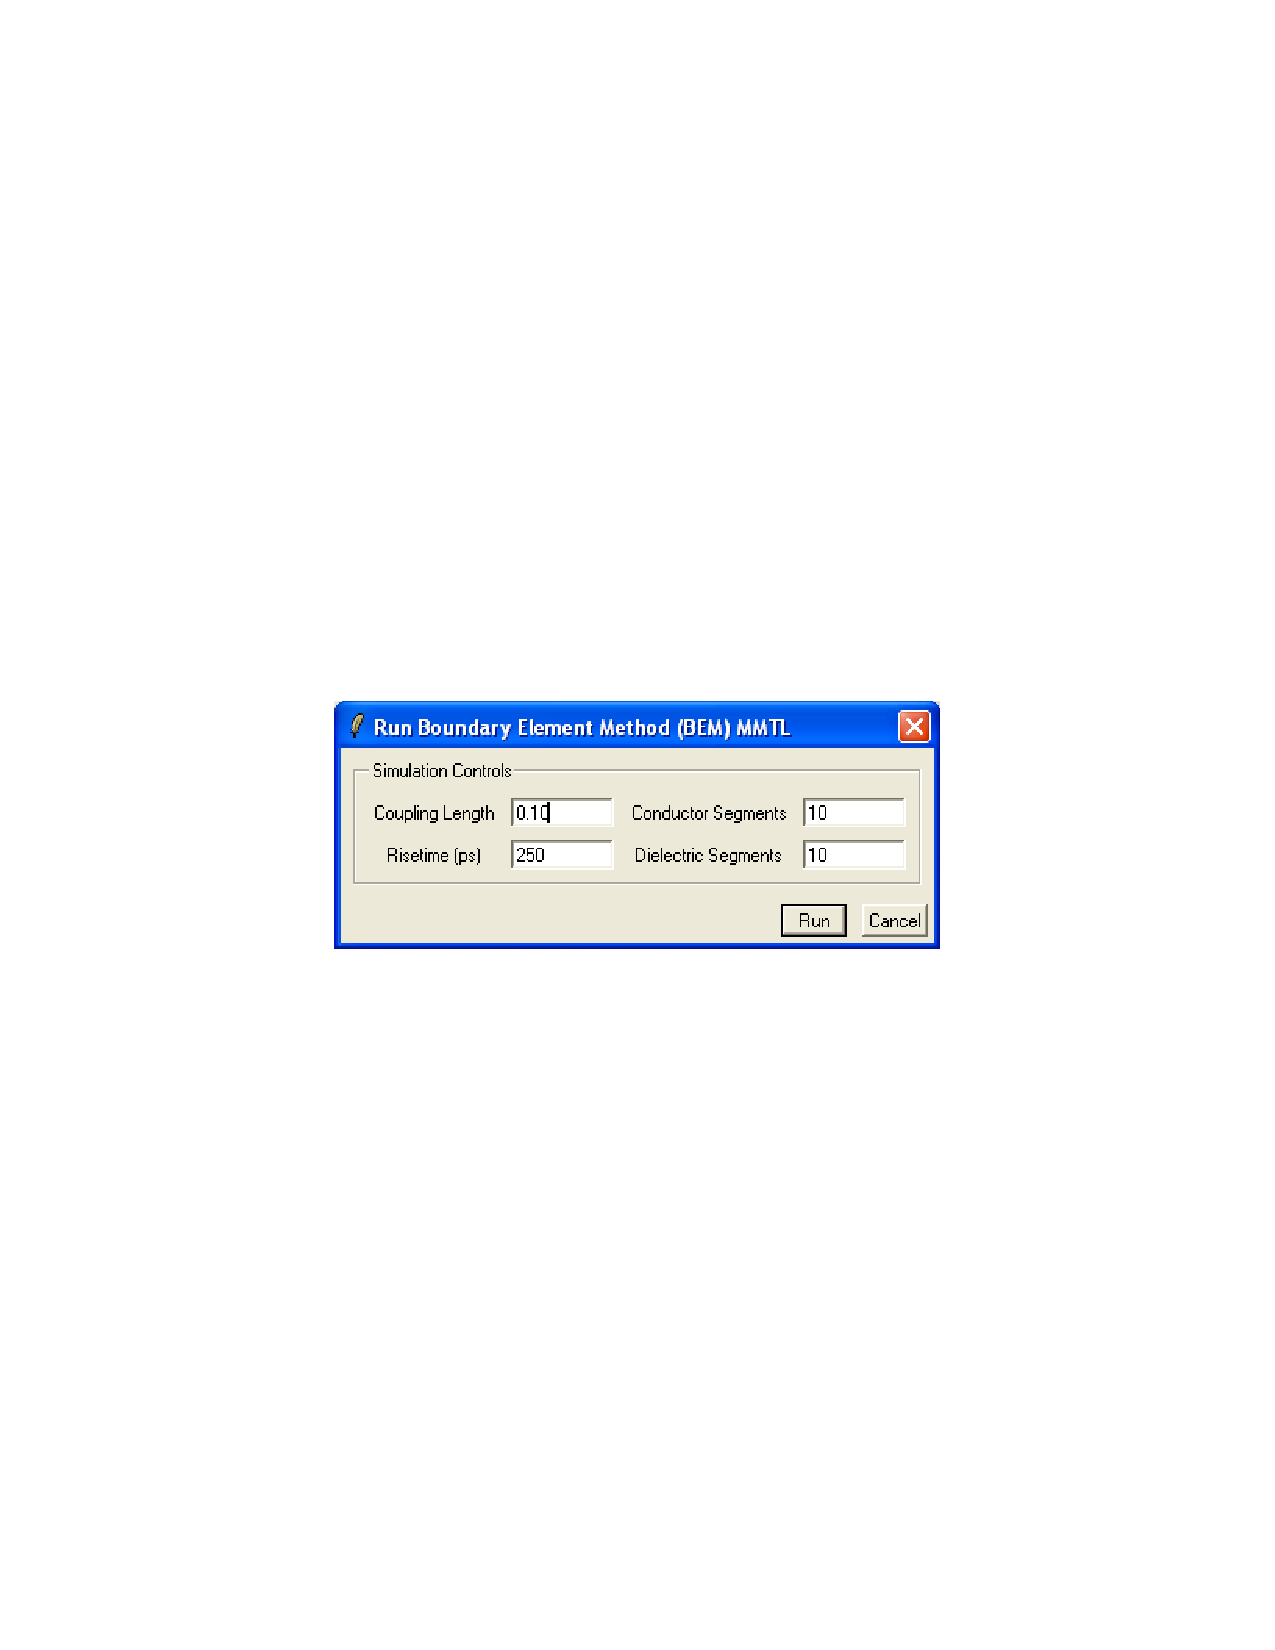
\includegraphics[scale=0.5]{mmtl-run}\end{center}
\caption { Running BEM MMTL }
\label{fig:mmtl-run}
\end{figure}


%-----------------------------------------------------------
%  Exporting HSPICE W-Element
%-----------------------------------------------------------

\subsection {Exporting HSPICE W-Element}

Choosing {\bf BEM $\Rightarrow$ Generate HSPICE W} from the menu will
generate a W-element model from the MMTL results.  The model file will
have the same name as your cross section file, with the extension {\tt
.hspice-w.rlgc}.  TNT will open a new window to show you the generated
W-element model.  You can cut and paste from this window, or refer to
the generated file from other applications.

The W-element file contains a comment header that describes the
original cross section and MMTL run.  Matrices $L_0$ and $C_0$ are
copied directly from MMTL's inductance and electrostatic induction
matrices.

Conductor losses, $R_0$ and $R_S$ are estimated from the conductor
geometries and materials properties, with these formulations.

\begin{equation}
R_0 = R_{DC} = \frac {1} {\sigma C_\text{Area}} \; \Omega/m
\end{equation}

\begin{equation}
R_S = R_{AC} = \frac {\sqrt{ \pi \mu_0 / \sigma}} {C_\text{Circum}} \; H/m
\end{equation}

Where $\sigma$ is the conductivity, $C_\text{Area}$ is the conductor
area, $C_\text{Circum}$ is the conductor circumference, and $\mu_0$ is
the permeability of free space.


%-----------------------------------------------------------
%  Parameter Sweep
%-----------------------------------------------------------

\subsection {Parameter Sweep}

TNT can run BEM MMTL iteratively, sweeping one or more parameters
through a range of values.  Choosing {\bf Sweep $\Rightarrow$ Sweep
Simulation} from the menu will allow you to choose the parameters to
be swept, from a dialog similar to that shown in
Figure~\ref{fig:sweep-select}.  Note that you can select any number of
parameters, including the simulation control parameters normally found
on the BEM MMTL simulation control dialog shown in
Figure~\ref{fig:mmtl-run}.

\begin{figure}[hbt]
\begin{center}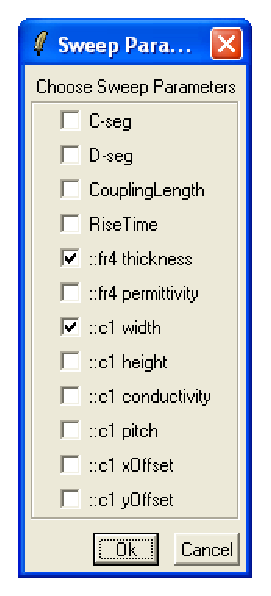
\includegraphics[scale=0.5]{sweep-select}\end{center}
\caption { Choosing BEM MMTL parameters to sweep }
\label{fig:sweep-select}
\end{figure}

Once you have selected parameters to sweep, you must specify starting
and ending values and the number of iterations for each parameter.  A
dialog similar to Figure~\ref{fig:sweep-parameters} will allow you to
enter the controlling values.

\begin{figure}[hbt]
\begin{center}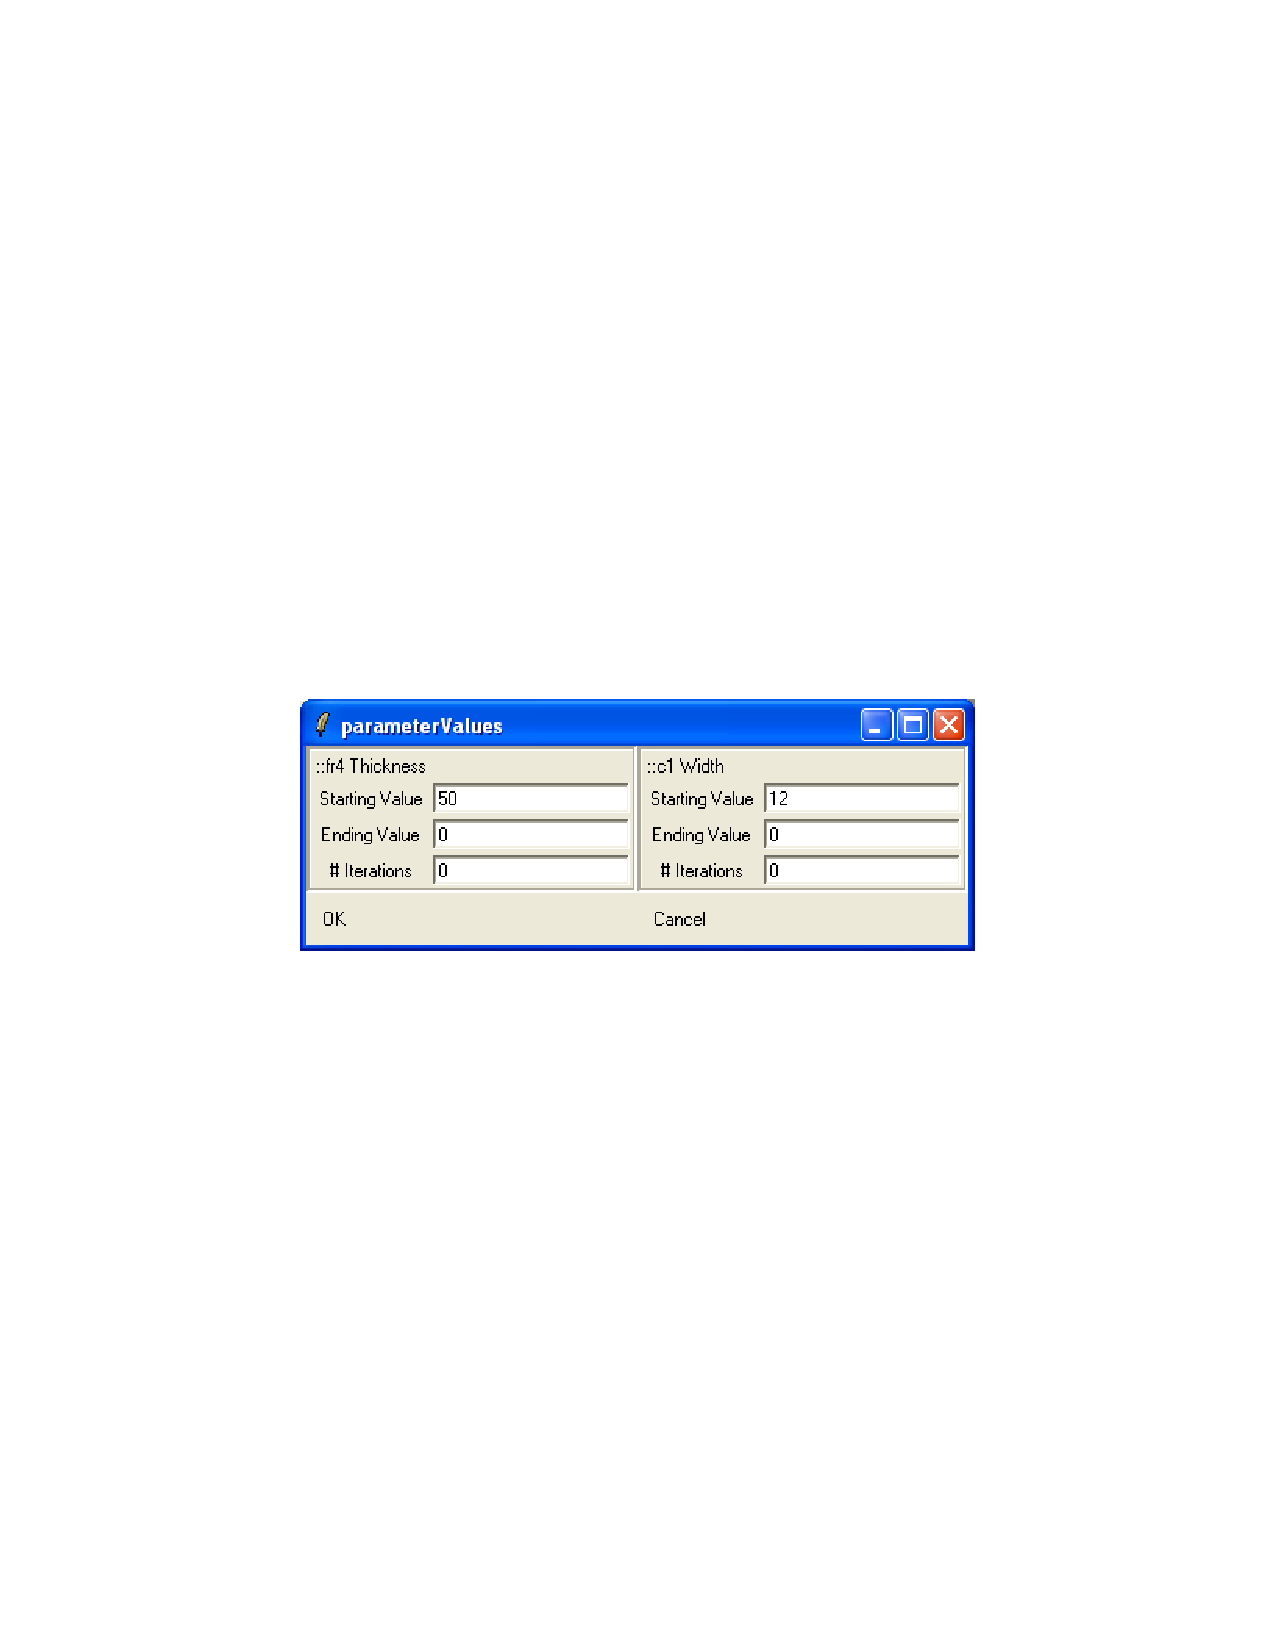
\includegraphics[scale=0.5]{sweep-parameters}\end{center}
\caption { Specifying BEM MMTL Sweep Ranges}
\label{fig:sweep-parameters}
\end{figure}

Sweeping several parameters can result in a very large number of
simulations.  TNT will run a comprehensive sweep, including $N$ runs,
where $N$ is the product of the number of iterations of each selected
parameter.  If you choose ten iterations of each of three different
parameters, you should expect 1000 MMTL runs.  TNT prompts you one
last time with the total number of iterations, to give you one last
chance to bail out.

Once the simulations are run, you can view the results of all the
simulations, or write a ``character separated file'' (sometimes called
a ``comma separated file'' or csv), which is suitable for import into
a spreadsheet program for analysis.  All parameters are exported to
the csv file.

%-----------------------------------------------------------
%  Iterating Conductor Width
%-----------------------------------------------------------

\subsection {Iterating Conductor Width}

Iteration is a specialized form of parameter sweep.  For some
transmission line designs, all layer thicknesses and materials
properties are fixed, and the engineer has control only over line
width.  The iteration feature of TNT allows you to specify these basic
cross section parameters, and then run MMTL iteratively until a
certain characteristic impedance is obtained.




%-----------------------------------------------------------
%  Wavelet Simulators
%-----------------------------------------------------------

\section {Wavelet Simulators}

TNT includes two prototype wavelet-based transmission line simulation
tools.  These tools use a simple finite element approach with Coifman
wavelet basis functions to compute full-wave transmission line
parameters.  You may choose either the ``RL'' calculator for
resistance and inductance, or the ``CAP'' calculator for capacitance.

The ``RL'' calculator dialog allows you to enter a number of frequency
points at which you would like the parameters computed.  The ``CAP''
calculator simply computes the line-to-line capacitance, which is
relatively independent of frequency.



%-----------------------------------------------------------
%  On-Line help
%-----------------------------------------------------------

\section {On-Line Help}

TNT includes online help in the form of this users guide and other
documentation.  The online help is displayed in a web browser.  On
Unix systems, TNT will attempt to run firefox, opera, mozilla, and
netscape, in that order, to display the files.  On Windows, TNT will
attempt to launch the default web browser on the document.

Printable versions of these documents are also available in TNT's {\tt
doc} directory, in portable document format (PDF).




%-----------------------------------------------------------
%  Acknowledgments
%-----------------------------------------------------------

\section {Acknowledgments} \label{sec:acknowledgements}

The authors would like to thank the engineers of Mayo SPPDG for their
patience, feedback, and technical support; Dr. George Pan of Arizona
State University and the students of his signal propagation laboratory
for algorithm research and prototype code; N. Naclario, Z. Lemnios,
D. Healy, D. Cochran, A. Krishnan, DARPA, and C. Hanson, SPAWAR/Code
8505, for program support.






\clearpage
\begin{thebibliography}{99}


\bibitem{Mayo-108} Pan, G-W, K. S. Olson, and B. K. Gilbert, {\em
Improved Algorithmic Methods For the Prediction of Wavefront
Propagation Behavior in Multiconductor Transmission Lines for High
Frequency Digital Signal Processors.} IEEE Transactions on
Computer-Aided Design of Integrated Circuits and Systems, 8(6)608-621
(June) 1989.


\bibitem{Mayo-131} Pan, G. W., J. A. Prentice, S. K. Zahn,
A. J. Staniszewski, W. L. Walters, and B. K. Gilbert, {\em The
Simulation of High-Speed, High-Density Digital Interconnects in Single
Chip Packages and Multichip Modules,} IEEE Transactions on Components,
Hybrids, and Manufacturing Technology, 15(4):465-477 (August) 1992.





\end{thebibliography}

\end{document}

